\section{Deadlocks}

A deadlock occurs because concurrent transactions hold and in turn request resources held by other transactions. 
\begin{definition}
    A \emph{lock graph} is a bipartite graph in which nodes are resources or transactions and arcs are lock requests or lock assignments. 

    A \emph{wait-for graph} is a graph in which nodes are transactions and arcs are waits for relationships. 
\end{definition}
A deadlock is represented by a cycle in the wait-for graph of transactions. 
\begin{figure}[H]
    \centering
    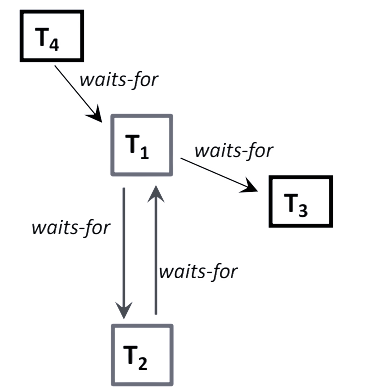
\includegraphics[width=0.35\linewidth]{images/waitgraph.png}
    \caption{An example of deadlock in the wait-for graph}
\end{figure}
It is possible to solve deadlocks in three different ways: 
\begin{itemize}
    \item Timeout: a transaction is killed and restarted after a given amount of waiting, to be determined by the system manager. 
    \item Deadlock prevention: kills transactions that could cause cycles. It is implemented in two ways: 
        \begin{enumerate}
            \item Resource-based prevention puts restrictions on lock requests. The idea is that every transaction requests all resources at once, and only once. The main problem
                is that it's not easy for transactions to anticipate all requests. 
            \item Transaction-based prevention puts restrictions on transactions' IDs. Assigning IDs to transactions incrementally allows to give an age to each one. It is 
                possible to choose to kill the holding transaction (preemptive) or the requesting one (non-preemptive). The main problem is that the number of killings is too big. 
        \end{enumerate}
    \item Deadlock detection: it can be implemented with various algorithms and used for distributed resources. 
\end{itemize}
\begin{definition}
    The \emph{distributed dependency graph} is a wait-for graph where external call nodes represent a sub-transaction activating another sub-transaction at a different node. 
\end{definition}
The arrow shows a wait-for relation among local transactions. If one term is an external call, either the source is waited for by a remote transaction or waits for a remote 
transaction. The Obermarck's algorithm needs the following assumptions: 
\begin{itemize}
    \item Transactions execute on a single main node. 
    \item Transactions may be decomposed in sub-transactions running on other nodes. 
    \item When a transaction spawns a sub-transaction it suspends work until the latter completes. 
    \item Two wait-for relationships:
        \begin{itemize}
            \item $T_i$ waits for $T_j$ on the same node because $T_i$ needs a datum locked by $T_j$. 
            \item A sub-transaction of $T_i$ waits for another sub-transaction of $T_i$ running on a different node. 
        \end{itemize}
\end{itemize}
The goal of this algorithm is to detect a potential deadlock looking only at the local view of a node. Nodes exchange information and update their local graph based on the 
received information. Node $A$ sends its local info to a node $B$ only if: it contains a transaction $T_i$ that is waited for from another remote transaction and waits for a 
transaction $T_j$ active on $B$ and $i>j$.
\begin{example}
    Given the following distributed dependency graph: 
    \begin{figure}[H]
        \centering
        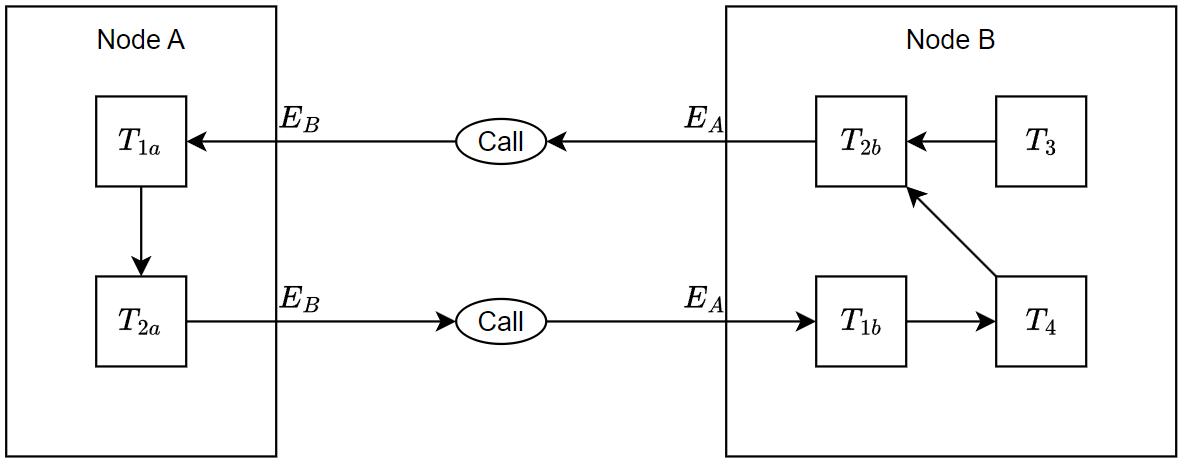
\includegraphics[width=0.5\linewidth]{images/distributedgraph.png}
    \end{figure}
    We can see that the potential deadlock is given by cycles. In this case, we have that $T_{2a}$ waits for $T_{1a}$ (data lock) that waits for $T_{1b}$ (call) that waits for 
    $T_{2b}$ (data locks) that waits for $T_{2a}$ (call). 
    
    In this case the node $A$ dispatches information to $B$, in fact we have $ E_b \rightarrow T_2 \rightarrow T_1 \rightarrow E_b$ and node $B$ cannot dispatch information to 
    $A$, because the forwarding rule is not respected: $E_a \rightarrow T_1 \rightarrow T_2 \rightarrow E_a$. 
\end{example}
The Obermarck's algorithm runs periodically at each node and consists in four steps: 
\begin{enumerate}
    \item Get graph info from the previous nodes.
    \item Update the local graph by merging the received information. 
    \item Check the existence of cycles among transactions denoting potential deadlocks: if found, select one transaction in the cycle and kill it. 
    \item Send updated graph info to the next nodes. 
\end{enumerate}
\begin{example}
    Given the following distributed system:
    \begin{figure}[H]
        \centering
        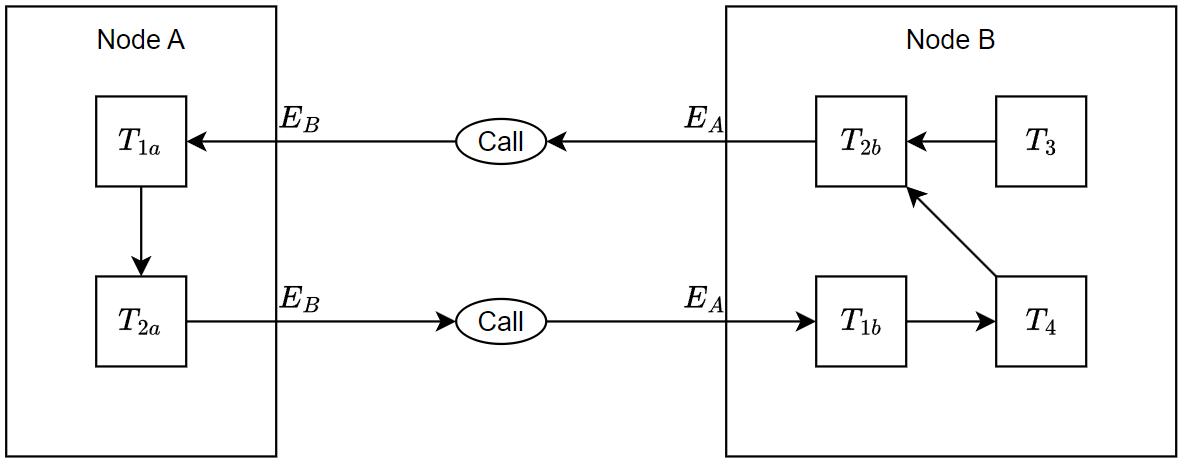
\includegraphics[width=0.5\linewidth]{images/distributedgraph.png}
    \end{figure}
    We want to apply the Obermarck's algorithm: 
    \begin{enumerate}
        \item Use the forwarding rule, in this case we have: 
            \begin{itemize}
                \item At Node $A$: $E_b \rightarrow T_2 \rightarrow T_1 \rightarrow E_b$ info sent to Node $B$
                \item At Node $B$: $E_a \rightarrow T_1 \rightarrow T_2 \rightarrow E_a$ info not sent $(i<j)$. 
            \end{itemize}
        \item At node $B$ there is the updated info $E_b \rightarrow T_2 \rightarrow T_1 \rightarrow E_b$ and it is added to the wait-for graph.
        \item At node $B$ a deadlock is detected (cycle between $T_1$ and $T_2$) and $T_1$, $T_2$ or $T_4$ are killed. 
        \item Updated information are sent to all nodes. 
    \end{enumerate}
\end{example}
There are four variants of this algorithm, based on various conventions.
\begin{table}[H]
    \centering
    \begin{tabular}{c|cc|}
    \cline{2-3}
    \textbf{}               & \textbf{Message condition} & \textbf{Message receiver} \\ \hline
    \multicolumn{1}{|l|}{A} & $i>j$                      & Following node            \\
    \multicolumn{1}{|l|}{B} & $i>j$                      & Preceding node            \\
    \multicolumn{1}{|l|}{C} & $i<j$                      & Following node            \\
    \multicolumn{1}{|l|}{D} & $i<j$                      & Preceding node            \\ \hline
    \end{tabular}
\end{table}
In practice, the probability of deadlocks ($n^{-2}$) is much less than the conflict probability ($n^{-1}$). There are techniques to limit the frequency of deadlocks: 
\begin{itemize}
    \item Update lock: the most frequent deadlock occurs when two concurrent transactions start by reading the same resources and then decide to write and try to upgrade their 
    lock to write on the resource. To avoid this situation, systems offer the update lock, that is used by transactions that will read and then write. The lock table become: 
    \begin{table}[H]
        \centering
        \begin{tabular}{ccccc}
        \textbf{}                                     & \multicolumn{4}{c}{\textbf{Resource status}}                                                                                                        \\ \cline{2-5} 
        \multicolumn{1}{c|}{\textbf{Request}}         & \textit{FREE}                     & \textit{SHARED}                   & \textit{UPDATE}                   & \multicolumn{1}{c|}{\textit{EXCLUSIVE}} \\ \hline
        \multicolumn{1}{|c|}{\textit{Shared lock}}    & \multicolumn{1}{c|}{$\checkmark$} & \multicolumn{1}{c|}{$\checkmark$} & \multicolumn{1}{c|}{$\checkmark$} & \multicolumn{1}{c|}{$\tikzxmark$}       \\ \hline
        \multicolumn{1}{|c|}{\textit{Update lock}}    & \multicolumn{1}{c|}{$\checkmark$} & \multicolumn{1}{c|}{$\checkmark$} & \multicolumn{1}{c|}{$\tikzxmark$} & \multicolumn{1}{c|}{$\tikzxmark$}       \\ \hline
        \multicolumn{1}{|c|}{\textit{Exclusive lock}} & \multicolumn{1}{c|}{$\checkmark$} & \multicolumn{1}{c|}{$\tikzxmark$} & \multicolumn{1}{c|}{$\tikzxmark$} & \multicolumn{1}{c|}{$\tikzxmark$}       \\ \hline
        \end{tabular}
    \end{table}
    \item Hierarchical lock: locks can be specified with different granularities. The objective of this is to lock the minimum amount of data and recognize conflicts as soon as
    possible. The method used to do so consists in asking locks on hierarchical resources by requesting resources top-down until the right level is obtained and releasing 
    locks bottom-up. This is done by using five locking modes: shared, exclusive, ISL (intention of locking a sub-element of the current element in shared mode), IXL (intention 
    of locking a sub-element of the current element in exclusive mode), and SIXL (lock of the element in shared mode with intention of locking a sub-element in exclusive mode). 
    The lock table become: 
    \begin{table}[H]
        \centering
        \begin{tabular}{ccccccc}
        \textbf{}                             & \multicolumn{6}{c}{\textbf{Resource status}}                                                                                                                                                                            \\ \cline{2-7} 
        \multicolumn{1}{c|}{\textbf{Request}} & \multicolumn{1}{c|}{\textit{FREE}} & \multicolumn{1}{c|}{\textit{ISL}} & \multicolumn{1}{c|}{\textit{IXL}} & \multicolumn{1}{c|}{\textit{SL}}  & \multicolumn{1}{c|}{\textit{SIXL}} & \multicolumn{1}{c|}{\textit{XL}}  \\ \hline
        \multicolumn{1}{|c|}{\textit{ISL}}    & \multicolumn{1}{c|}{$\checkmark$}  & \multicolumn{1}{c|}{$\checkmark$} & \multicolumn{1}{c|}{$\checkmark$} & \multicolumn{1}{c|}{$\checkmark$} & \multicolumn{1}{c|}{$\checkmark$}  & \multicolumn{1}{c|}{$\tikzxmark$} \\ \hline
        \multicolumn{1}{|c|}{\textit{IXL}}    & \multicolumn{1}{c|}{$\checkmark$}  & \multicolumn{1}{c|}{$\checkmark$} & \multicolumn{1}{c|}{$\checkmark$} & \multicolumn{1}{c|}{$\tikzxmark$} & \multicolumn{1}{c|}{$\tikzxmark$}  & \multicolumn{1}{c|}{$\tikzxmark$} \\ \hline
        \multicolumn{1}{|c|}{\textit{SL}}     & \multicolumn{1}{c|}{$\checkmark$}  & \multicolumn{1}{c|}{$\checkmark$} & \multicolumn{1}{c|}{$\tikzxmark$} & \multicolumn{1}{c|}{$\checkmark$} & \multicolumn{1}{c|}{$\tikzxmark$}  & \multicolumn{1}{c|}{$\tikzxmark$} \\ \hline
        \multicolumn{1}{|c|}{\textit{SIXL}}   & \multicolumn{1}{c|}{$\checkmark$}  & \multicolumn{1}{c|}{$\checkmark$} & \multicolumn{1}{c|}{$\tikzxmark$} & \multicolumn{1}{c|}{$\tikzxmark$} & \multicolumn{1}{c|}{$\tikzxmark$}  & \multicolumn{1}{c|}{$\tikzxmark$} \\ \hline
        \multicolumn{1}{|c|}{\textit{XL}}     & \multicolumn{1}{c|}{$\checkmark$}  & \multicolumn{1}{c|}{$\tikzxmark$} & \multicolumn{1}{c|}{$\tikzxmark$} & \multicolumn{1}{c|}{$\tikzxmark$} & \multicolumn{1}{c|}{$\tikzxmark$}  & \multicolumn{1}{c|}{$\tikzxmark$} \\ \hline
        \end{tabular}
    \end{table}
    \begin{example}
        Given a table $X$ with eight tuples divided in two pages: 
        \begin{table}[H]
            \centering
            \begin{tabular}{cc}
            \textbf{P1}                 & \textbf{P2}               \\ \hline
            \multicolumn{1}{|c|}{$t1$}  & \multicolumn{1}{c|}{$t5$} \\ \hline
            \multicolumn{1}{|c|}{$t2$}  & \multicolumn{1}{c|}{$t6$} \\ \hline
            \multicolumn{1}{|c|}{$t3$}  & \multicolumn{1}{c|}{$t7$} \\ \hline
            \multicolumn{1}{|c|}{$t4$}  & \multicolumn{1}{c|}{$t8$} \\ \hline
            \end{tabular}
        \end{table}
        And two transactions with the following schedules: 
        \[T_1=r(P1)\:w(t3)\:r(t8)\]
        \[T_2=r(t2)\:r(t4)\:w(t5)\:w(t6)\]
        We can see that they are not in a read-write conflict (because they are independent of the order). Without hierarchical locking both transactions needs to operate on the 
        same table, so the concurrency will be almost useless in this case. But with this technique, calling $X$ the table, we have that the transaction acquires the following
        locks: 
        \[T_1:\:IXL(root)\:SIXL(P1)\:XL(t3)\:ISL(P2)\:SL(t8)\]
        \[T_2:\:IXL(root)\:ISL(P1)\:SL(t2)\:SL(t4)\:IXL(P2)\:XL(t5)\:XL(t6)\]
    \end{example}
\end{itemize}